\documentclass{article}

\usepackage{amsmath}
\usepackage{graphicx}
\usepackage{hyperref}
\usepackage[utf8]{inputenc}
\usepackage{lipsum}
\usepackage{multicol}
\usepackage{titling}
\usepackage[a4paper]{geometry}
\usepackage{tikz}
\geometry{
    left=20mm,
    top=20mm,
}
\renewcommand{\thesection}{\Roman{section}}
\renewcommand{\thesubsection}{\Roman{subsection}}
\title{\LARGE \textbf {\huge{Tugas Probabilitas dan Statistika\\}
}
    Ditulis dalam \textbf{\LaTeX}
}
\author{
    M Rizqi R\\
    20051204034\\
    Teknik Informatika 2020 B\\
    Universitas Negeri Surabaya\\
}
\date{\today}

\begin{document}
    \maketitle
    \begin{multicols*}{2}
    \section{}
    \textbf{Variabel\\}
    M = Medical 
    N = Non-Medical
    P = Pria\\
    W = Wanita
    A = Anak-Anak
    D = Dewasa
    \hfill \break
    \textbf{Data: \\}
    $n(s) = 20.000$\\
    (I)     $n(P \cap M) = 3.000$\\ 
    (II)    $n(M \cap A) = 2.500$\\
    (III)   $n(P \cap A) = 3.000$\\
    (IV)   $n(M \cap (P \cap A)) = 1.000$\\
    (V)         $n(M)=5000$\\
    (VI)        $n(B)=10.000$\\
    (VII)       $n(A)=12.000$\\
    \textbf{Ditanya =} $n(W \cap(D \cap M))$?\\
    \hfill\break
    Jawab :
    \begin{enumerate}
        \item $n(W) = n(S)-n(P)=20.000-10.000=10.000$
        \item $n(D) = n(S)-n(A)=20.000-12.000=8000$
        \item $n(P \cap N) = 20.000 - 5000=15.000$
        \item $n(W \cap M) = n(M) - n(P\cap M) = 5000-3000=2000$
        \item $n(M \cap D) = n(M)-n(M \cap A) = 5000-2.500=2.500$
        \item $n(W \cap D) = n(D)-n(P \cap D) = 8000-7000=1000$
        \item $n(M \cap (P \cap A)) = 1000$
        \item $n(M \cap (W \cap A)) =n(M \cap A)-n(M \cap (P \cap A))=
        2.500-1000= 1.500$ 
        \item $n(W \cap (P \cap M)) = n(W \cap M)-n(M \cap(W \cap A))
        =2000-1.500=500$ \end{enumerate}
    \section{}
    \textbf{Variabel\\}
    S = Himpunan Semesta\\
    P = Perokok\\
    K = Alkohol\\
    G = Gaya hidup tidak sehat\\
    \textbf{Data: \\}
    \begin{enumerate}
        \item \( n(S) = 40.000\)
        \item \( n(P) = 29.000\)
        \item \( n(K) = 25.000\)
        \item \( n(G) = 30.000\)
        \item \( n(P \cap K) = 22.000\)
        \item \( n(P \cap G) = 24.000\)
        \item \( n(K \cap K) = 20.000\)
        \item \( n(P \cap K \cap G) = 20.000\)
    \end{enumerate}
    Perokok tapi tidak kecanduan alkohol = \( n(K^c \cap (A-B)^c)\)\\
    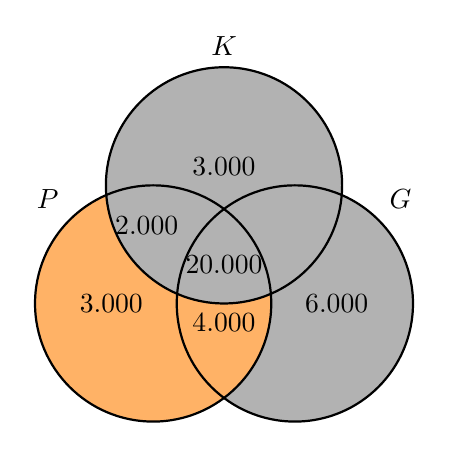
\begin{tikzpicture}
        [thick,
        set/.style = {circle,
        minimum size = 3cm,
        fill=black!30}]
 
        % Set A
        \node[set,label={135:$P$},fill=orange!60] (P) at (0,0) {};

        % Set B
        \node[set,label={45:$G$}] (G) at (1.8,0) {};

        % Set C
        \node[set,label=$K$] (K) at (0.9,1.5) {};

        % Intersection
        \begin{scope}
            \clip (0,0) circle(1.5cm);
            \clip (1.8,0) circle(1.5cm);
            \fill[orange!60](0,0) circle(1.5cm);
        \end{scope}
        \begin{scope}
            \clip (0,0) circle(1.5cm);
            \clip (1.8,0) circle(1.5cm);
            \clip (0.9,1.5) circle(1.5cm);
            \fill[black!30](0,0) circle(1.5cm);
        \end{scope}

        \node at (barycentric cs:P=1)[left]{$3.000$};
        \node at (barycentric cs:P=1,K=1)[above left]{$2.000$};
        \node at (barycentric cs:P=1,G=1)[below]{$4.000$};
        \node at (barycentric cs:G=1)[right]{$6.000$};
        \node at (barycentric cs:K=1)[above]{$3.000$};
        \node at (barycentric cs:P=1,G=1,K=1 ){$20.000$};

        % Circles outline
        \draw (0,0) circle(1.5cm);
        \draw (1.8,0) circle(1.5cm);
        \draw (0.9,1.5) circle(1.5cm);
    \end{tikzpicture}
        \hfill \break
       Jadi, \( n(K^c \cap (A-B)^c)\)\\
       $= 4000+3000\\$
        \colorbox{orange!60}{$=7000$ pasien}
    \end{multicols*}
    
\end{document}













